%!TEX TS-program = xelatex
\documentclass[]{friggeri-cv}
\usepackage{afterpage}
\usepackage{hyperref}
\usepackage{ucs}
\usepackage[utf8x]{inputenc}
\usepackage{color}
\usepackage{xcolor}
\hypersetup{
    pdftitle={Colin LEVERGER},
    pdfauthor={Colin LEVERGER},
    pdfsubject={CV},
    pdfkeywords={CV, Colin LEVERGER, young Data \& DevOps Engineer},
    colorlinks=false,       % no lik border color
    allbordercolors=white    % white border color for all
}
% \addbibresource{bibliography.bib}
\RequirePackage{xcolor}
\definecolor{pblue}{HTML}{4CAF50}

\begin{document}
\header{Colin}{LEVERGER}
      {Ph. D. - Data Engineer \& DevOps}

% Fake text to add separator      
\fcolorbox{white}{gray}{\parbox{\dimexpr\textwidth-2\fboxsep-2\fboxrule}{%
.....
}}

% In the aside, each new line forces a line break
\begin{aside}
  
\includegraphics[scale=0.01]{img/white.png}
  \section{Adresse}
    Centre ville 
    35000 RENNES 
    FRANCE
    ~
  \section{Tel}
    +33 (0)6 30 83 62 59 
    ~
  \section{Mél.}
    \href{mailto:colin.leverger@orange.fr}{\textbf{colin.leverger@}\\orange.fr}
  \section{Web \& Git}
    \href{http://www.colinleverger.fr}{colinleverger.fr}
    \href{https://www.linkedin.com/in/colinleverger}{lnkdin.me/cleverger}
    \href{https://github.com/ColinLeverger}{github/ColinLeverger}
    ~
  \section{Langages}
  \textbf{Principaux} :
  \emph{Python} : 4+ années
  \emph{Bash/Unix} : 6+ années
  \textbf{Secondaires} :
  \emph{Scala/Java} : 4 années
  \emph{HTML/PHP} : 4 années
  \emph{R} : 3 années
  \textbf{Déjà utilisés} :
  \emph{JavaScript} : 2 années
  \emph{SQL }: 1 an
  %\textbf{Interests \& curiosity}
  %\emph{R}: few projects
  ~
  \section{Langues}
  \textbf{Français} : natif
  \textbf{Anglais} : C1+
  ~
  \section{DevOps exp.}
  \emph{Docker} : 4+ années
  \emph{Outils CI} : 3+ années
  \emph{GCP/k8s} : 1+ années
  \emph{Ansible} : 1 an
  \emph{OpenStack} : 1 an
  \emph{ELK} : 1 an
  %\emph{JMeter}: 1 year
    ~
  \section{Intérêts pro.}
  Data Science, 
  données massives, 
  intégration continue,
  cybersécurité, etc...
  ~
  \section{Soft skills}
  Autonomie
  Passion
  Curiosité
  Méthode
  Communication 
  Créativité
  Ténacité
  %\hspace*{-1.3in}
  %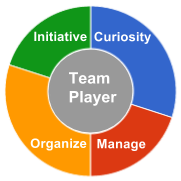
\includegraphics[scale=0.55]{img/personal.png}
    ~
\end{aside}

\section{Expériences}
\begin{entrylist}
  \entry
  {01/21 - actuel}
  {Data Engineer}
  {\href{http://www.orange.com/en/home}{Orange Labs \& Services}, Rennes - FRANCE}
  {
    Travail dans une équipe de développeurs expérimentés sur des problématiques de Data Engineering. 
    Développement de solutions Cloud (GCP) en Python pour faciliter le travail des équipes (Data Scientists \& developpeurs).
    Sujets couverts variés (cybersécurité, outillage technique, conduite de projet, communications en anglais avec prestataires, recherche sur des modèles de machine learning/Data Science, etc.). 
    Encadrement d’une stagiaire ingénieure. Implication dans la vie de l’équipe (ambassadeur sur site, entre autres).  
  }
  \entry
    {10/17 - 11/20}
    {Doctorant}
    {\href{http://www.orange.com/en/home}{Orange Labs \& Services}, Rennes - FRANCE}
    {
    Recherche dans le domaine du planning capacitaire.
    Développement d’algorithmes d’apprentissage automatique avec Python, Pandas, R, Keras \& DeepAR, et analyse de séries temporelles pour prédire les performances des infrastructures.
    Localisation conjointe au laboratoire INRIA et à Orange Labs.
    Publication de trois papiers de recherche dans des conférences nationales et internationales (détails disponibles sur demande).
    }
  \entry
    {02/19 - 05/19}
    {Chercheur détaché}
    {National Institute of Technology, Tokyo - JAPON}
    {Expérience de recherche de trois mois au laboratoire NII à Tokyo.
    Développement d'un dashboard R Shiny pour afficher de nombreuses séries temporelles.
    Initiation d'une toute nouvelle collaboration de recherche.
    }
       % \vspace{-1.1em}
  \entry
    {09/17 - 11/18}
    {Assistant de laboratoire}
    {Université de Rennes 1 and E.N.S.A.I., Rennes - FRANCE}
    {88 h comme assistant de laboratoire à l'Université de Rennes 1 et E.N.S.A.I. Rennes pour étudiants de licence et master.
    Création et encadrement d'un nouveau sujet de TP Python.% basé sur une application de scrapping en Python 3.
    }
  \entry
    {09/14 - 09/17}
    {Apprenti Ingénieur Logiciel}
    {\href{http://www.orange.com/en/home}{Orange Labs \& Services}, Rennes - FRANCE}
    {Apprentissage pour développer un logiciel pour le test automatique des infrastructures d’Orange, en Scala et en Bash, tout en suivant une méthodologie DevOps. Travail dans une équipe de 14 experts métrologues. 
    % Utilisation d’outils de tests comme Gatling et Jmeter pour stresser les infrastructures.
    % Expérimentations avec la stack ELK, Grafana et influxdb pour le traitement d’une masse importante de logs.
    Développement d’algorithmes d’apprentissage automatique pour le planning capacitaire.
    Utilisation de Scala, Spark, Elasticsearch, Logstash, Kibana, R, Openstack, influxdb, Gatling, Jmeter, etc.    
}
  \entry
    {02/15 - actuel}
    {Ingénieur système et réseaux (loisir)}
    {Rennes - FRANCE}
    {Gestion de mon serveur dédié.
    Utilisation de Docker pour gérer les services virtuels, Jenkins pour faire de l'intégration continue, Ansible pour scripter la configuration des serveurs. Expérimentations avec la stack ELK et Grafana pour monitorer services et cyberattaques.    
   }
%  \entry
%    {04/14 - 07/14}
%    {Internship}
%    {\href{http://www.ait.ie/}{Athlone Institute of Technology}, Athlone - IRELAND}
%    {Three months end-of-course internship; preparation of project subjects for students. Worked with \emph{Arduino}, \emph{Java}, \emph{HTML/CSS}, \emph{PHP} and \emph{C}.}
\end{entrylist}

\vspace{-1.1em}

%\section{Research \& Publications}
%\begin{entrylist}
%  \entry
%    {10/19}
%    {IDEAL Conference (C)}
%    {Manchester - UNITED KINGDOM}
%    {"Toward a framework for seasonal time series forecasting using clustering.", Leverger, C., Malinowski, S., Guyet, T., Lemaire, V., Bondu, A., \& Termier, A.}
%  \entry
%    {09/18}
%    {AALTD workshop at ECML (A)}
%    {Dublin - IRELAND}
%    {"Day-ahead time series forecasting : application to capacity planning.", Leverger, C., Lemaire, V., MaliMaintenantski, S., Guyet, T., \& Rozé, L.}
%\end{entrylist}

\section{Formation}
\begin{entrylist}
  \entry
    {09/16 - 02/17}
    {ERASMUS}
    {\href{http://www.ruc.dk/en/}{Roskilde University}, Roskilde - DANEMARK}
    {
    ERASMUS au Danemark pendant 5 mois pour le dernier semestre académique.
    \underline {Sujets principaux} : architecture IT, design de logiciels centrés utilisateurs, sécurité, Big Data, danois.
    }
  \entry
    {09/14 - 09/17}
    {Diplôme d'ingénieur}
    {\href{http://www.enssat.fr}{E.N.S.S.A.T.}, Lannion - FRANCE}
    {Études d’ingénieur en informatique, multimédia et réseaux. \underline {Sujets principaux} : applications réseau, architecture des systèmes, design de services et d’interfaces utilisateur. Participation à de nombreux projets de développement logiciel, certains étant disponibles sur mon portfolio \href {https://colinleverger.fr}{https://colinleverger.fr}
}
  %\entry
  %  {2012 - 2014}
  %  {Two year Undergraduate University Degree of Technology in Electronics and Computing}
  %  {\href{https://iut-rennes.univ-rennes1.fr/les-6-departements/genie-electrique-informatique-industrielle}{Universit\'e de Rennes 1}, Rennes - FRANCE}
  %  {Main subjects: Programming, Microchip, Digital and Analogic Electronics.}
\vspace{-1.2em}  
  %\entry
  %  {2016  -  2017}
  %  {MOOCs and online courses}
  %  {Coursera and edX, e-learning}
  %  {Learning Functional paradigm with the Scala language. The course is complemented by a series programming projects as homework assignments. Learning Google Cloud Platform: SDKs \& CLI, VMs management, Scalability, ...}
\end{entrylist}

\vspace{-1.1em}

%\section{Certifications}
%\begin{entrylist}
%  \entry
%    {07/16 - 02/17}
%    {Scala Specialization}
%    {Coursera, E-learning}
%    {Learning Functional paradigm with the Scala language. The course is complemented by a series programming projects as homework assignments.}
  %\entry
  %  {01/17 - 02/17}
  %  {Google Cloud Platform Specialization}
  %  {Coursera, E-learning}
  %  {Learning Google Cloud Platform: SDKs \& CLI, VMs management, Scalability, ...}
%\end{entrylist}

\section{Compétences}

\begin{entrylist}
%  \entry
%    {Computing}
%    {Languages}
%    {}
%    {Python, R, Scala, Java, C, HTML/CSS, PHP, JavaScript, Bash/scripting, SQL, NoSQL, \LaTeX}
  \entry
%    {}
    {Informatique}
%    {Paradigms}
%    {}
%    {Functional, imperative, object-oriented, concurrent programming, real-time programming}
%  \entry
%    {}
    {Outils notables}
    {}
    {FastAPI, Gitlab-CI, Pandas, NumPy, scikit-learn, Tensorflow, Matplotlib, Jupyter Notebook, R, ggplot2, Git, Spark, influxDB, massive grid computing, Khiops coclustering tool @Orange}
  \entry
    {Hobbies}
    {MOOCs Coursera}
    {}
    {Spécialisation Scala, Data Engineering Google Cloud Platform, etc.}
    % \entry
    % {}
    % {Musique}
    % {}
    % {Musicien, membre d’un groupe où nous interprétons des créations originales en live et où nous produisons et diffusons nos musiques. Gestion du projet, du démarchage et de la communication du groupe.
    % }

  \entry
    {}
    {Sport}
    {}
    {Ashtanga Yoga, niveau intermédiaire. Coureur, grimpeur et nageur régulier.}
\end{entrylist}
\end{document}